%%%%%%%%%%%%%%%%%%%%%%%%%%%%%%%%%%%%%%%%%%%%%%%%%%%
% physvaltools.tex
%%%%%%%%%%%%%%%%%%%%%%%%%%%%%%%%%%%%%%%%%%%%%%%%%%%
\label{sec:physvaltools}
\subsection{\textbf{Physics Validation Tools}}

\subsubsection{Physics Validation Procedure}
The accuracy of the \Gfour{} physics models is benchmarked regularly using thin-
and thick-target tests.  Thin-target tests allow a detailed study of specific
observables from a single physics process for a given configuration of
projectile particle type, projectile kinetic energy and target material.
A large set of published thin-target data, collected over several years, is 
used roughly once per month to validate each internal development release. 
These data can also be used for tuning some of the parameters of the physics
models.  This is particularly true for the hadronic models, many of which are 
phenomenological.

Thick-target tests are mainly based on test beam setups.  These tests allow the
assessment of the physics accuracy of \Gfour{} simulations in realistic 
configurations, which involve several physics processes and multiple energy 
scales.  A notable example is the measurement of the properties of 
electromagnetic and hadronic showers in calorimeter test beam setups which were
carried out for the preparation of the LHC experiments, and which are ongoing
for the Linear Collider detector (CALICE).

Test beam simulations are in general complex and time-consuming, and are 
therefore repeated by experimentalists only for some \Gfour{} public releases.
To get more frequent and regular feedback, \Gfour{} developers have created a
set of simplified test beam setups which are used for regression testing, that 
is, the comparison of two or more versions of \Gfour{} for any observable.  
When a statistically significant difference is detected, for instance if the 
hadronic shower becomes wider than that observed in a previous \Gfour{} version,
the code changes responsible for the difference are investigated.

\subsubsection{Physics Validation Tests}
Model development and improvement work is tightly coupled with extensive 
efforts to validate \Gfour{} physics with experimental data.  A large collection 
of tests ranges from validation at the single process level and comparison with 
thin target experimental data to the validation of complete physics lists and 
comparison with results from LHC experiments.
 
In particular, validation with thin target data is crucial in judging the 
quality of model prediction and model tuning.  Thin target validations are done
for
\begin{itemize}
\item stopping particles ($\bar{p}$, $\pi^-$, $K^{-}$, $\Sigma^{-}$, $\Omega$),
\item low energy data ($<$100 MeV) with inclusive $n$, $p$ production in $n$,
      $p$, $\gamma$ beams on nuclear targets,
\item medium energy data (100 MeV-200 GeV) that includes $n$, $p$, $\pi^+$ 
      production in p-A or $\pi^{\pm}$-A interactions,
\item high energy data ($>$ 20 GeV) for inclusive hadron production in $\pi$ or
      $p$ interactions with nuclear targets, and
\item a number of comparisons for simplified yet realistic experimental setups
      by the \Gfour{} team and LHC experimentalists.
\end{itemize}

\subsubsection{Physics Validation Repository}
As the number of regularly performed validation tests increases and the 
collection of results grows, storing them and making them available to the 
user community becomes a challenge of its own.  It was decided to organize
this material in a central repository and to make this data generally and easily
available, not only for internal collaboration use, but also for the user 
community.

The Physics Validation Repository stores data in the form of images with 
meta-data, or as the raw data points from both simulation and experiment.
Meta-data includes descriptions of the tests, lists of references describing the
origin of the experimental data, and other parameters which describe the test,
such as beam particle type, its energy or momentum, the reaction observed and 
its secondaries, and the observable that is extracted from the measurement. 

The ability to store images allowed the initial population of the database with
the available collection of existing test results.  The alternative method of 
storing raw data points allows more interactivity, and can be used for example,
in performing regression testing and model comparisons.

As shown in Figure \ref{fig:webapp}, the physics validation repository consists
of a PostgresSQL database, a Java API and a JSP web application. 
The PostgresSQL \cite{PVT:postgres} relational database stores collections of 
tests, such as images, tags, descriptions, references, and images with meta-data
or raw data points, both experimental and simulated.
% The advantage over raw data points is
%that the use can select compatible data and overlay them and compare them. 
%This allows e.g. for the comparison of different \Gfour version
%(regression testing), comparison of different available models, target 
%materials  etc. 

The Java API is based on the data access object (DAO) design pattern, which  
provides an abstract interface to the database.  Using mapping application calls
to the persistence layer enables the DAO to provide some specific data 
operations without exposing details of the database.
% It 
%separates what data accesses the application needs, in terms of 
%domain-specific objects and data types (the public interface of the DAO), 
%from how these are implemented with the database schema.

The web application \cite{PVT:home} is based on the Enterprise Edition (Java EE)
\cite{PVT:javaee} of the Java Platform, deployed on a GlassFish Application
server \cite{PVT:glassfish}.  This allows tests to be viewed and modified, new 
tests to be uploaded, and provides security and authentication to grant access 
to functions and data internal to the \Gfour{} collaboration.
 
The PrimeFaces JSF (java server faces) Framework \cite{PVT:primefaces} is used
to create interactive, modern-looking web interfaces and charting tools based
on JavaScript are used for plotting.
% jfreechart java 
% library \cite{PVT:jfreechart} or the Highcharts 
% JavaScript library 
% \cite{PVT:highcharts} is used for plotting. 
%To convert data in the database into plots we make use of the jfreechart 
%java library or to create interactive charts we use the Highcharts JavaScript
%library. 

\begin{figure}[htb]
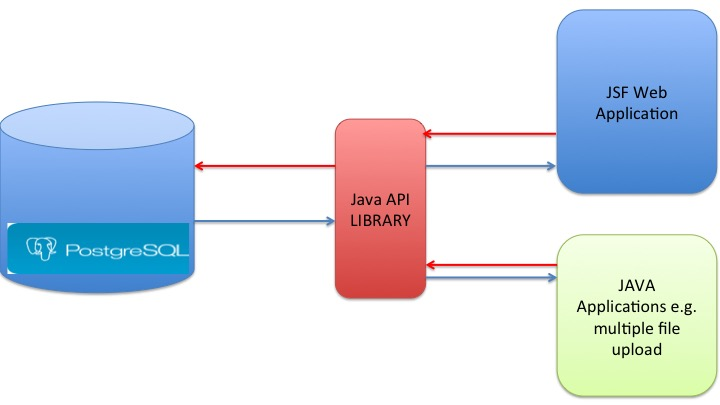
\includegraphics[width=0.45\textwidth]{figures/Components.jpg}
%  \centering
%  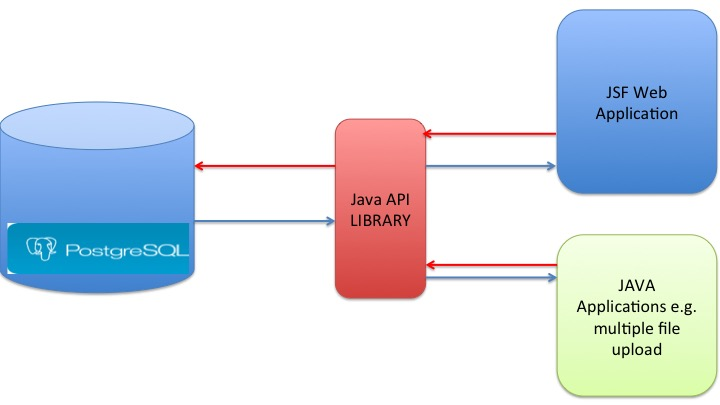
\includegraphics[width=3.4in]{figures/Components.jpg}
  \caption{Components of the \Gfour{} validation repository.} 
  \label{fig:webapp}
\end{figure}
